\documentclass[conference]{IEEEtran}
\IEEEoverridecommandlockouts

\usepackage{cite}
\usepackage{amsmath,amssymb,amsfonts}
\usepackage{algorithmic}
\usepackage{graphicx}
\usepackage{textcomp}
\usepackage{xcolor}
\def\BibTeX{{\rm B\kern-.05em{\sc i\kern-.025em b}\kern-.08em
    T\kern-.1667em\lower.7ex\hbox{E}\kern-.125emX}}

% ------ START Custom Section For "usepackage" ------

\usepackage{hyperref}
\usepackage{epigraph}
\usepackage{csquotes}
\usepackage{tikz}
\usepackage{xcolor}
\usepackage{svg}
\usepackage{float} % Enables you to force a "floating object" like the environments 'figure' and 'table' inline with the text.
\usepackage{morefloats} % Enalbes LaTeX to exceed the maximum 18 floats in a document.
\usepackage{nameref}
\usepackage{wrapfig}
\usepackage{subcaption} % Enable pictures to be aligned side by side. NOT COMPATIBLE with adjustbox.
\usepackage{adjustbox}
\usepackage{cancel}
\usepackage{ulem}
\graphicspath{ {./images/} }

% packages for typesetting source-code
\usepackage{listings} % Required for inserting code snippets

% Optional packages
\usepackage{blindtext} % Sample text, false content, Lorem Ipsum type of random generated text.

% ------ END Custom Section For "usepackage" ------


% ------ START Custom Section For environment settings ------

\newenvironment{notes}[1][\unskip]
{
\par
\noindent
\textcolor{blue}{\bfseries{Notes - } #1:}
\\ \color{blue}}
{}

% \newenvironment{notes}[1]
%     {\begin{center}
%     #1\\[1ex]
%     \begin{tabular}{|p{50mm}|}
%     \hline\\
%     }
%     { 
%     \\\\\hline
%     \end{tabular} 
%     \end{center}
%     }

\newenvironment{followup}[1][\unskip]{%
\par
\noindent
\textcolor{red}{\bfseries{Follow-up - } #1!!!}
\\ \color{red}}
{}

\newenvironment{question}[1][\unskip]{%
\par
\noindent
\textcolor{orange}{\bfseries{Question - } #1???}
\\ \color{orange}}
{}

% Typesetting code snippets
% The code snippet typesetting below is based on https://www.latextemplates.com/template/code-snippet
% Original Author: This template was created for LaTeXTemplates.com by vel@latextemplates.com
\definecolor{DarkGreen}{rgb}{0.0,0.4,0.0} % Comment color
\definecolor{highlight}{RGB}{204,255,229} % Code highlight color
\definecolor{Gray}{RGB}{224,224,224}
\definecolor{Purple}{RGB}{255,0,255}
\definecolor{Blue}{RGB}{0,0,255}

% ------ END Custom Section For environment settings ------



\begin{document}

\title{Intrusion Detection Tools\\}

\author{\IEEEauthorblockN{Kim André Næss, Dale Peregrino Bada, Muhammad Javed Iqbal}
\IEEEauthorblockA{\textit{Cyber Security} \\
\textit{Noroff University College}\\
Kristiansand, Oslo, Norway \\
kim.naess@stud.noroff.no, dale.bada@stud.noroff.no, muhammad.iqbal@stud.noroff.no}
}


\maketitle

\begin{abstract}

This state-of-art review paper will examine the latest Intrusion Detection Systems (IDS) and Intrusion Prevention Systems (IPS) applicable for Small and Midsize Businesess (SMB), where SMB are as defined by Gartner.

This review has 3 key objectives. Firstly, it will define and identify what kind of network security threats are most prevalent and most urgent for SMBs' to address. Secondly, we will identify what open source software are available for SMBs' to manage and mitigate identified threats. Then in the third final part, we will review how these open source software addresses the identified network threats.

Each tools' features, capabilities, advantages and limitations will be compared. How each system fare with regards to manageability, cost effectiveness and return of investment, will also be taken into consideration. With all above parameters being equal, should be able to determine which IDS/IPS are most suitable for SMBs'. 

\end{abstract}

% \begin{abstract}
% Lorem ipsum dolor sit amet mollit sunt duis velit non aliquip in labore minim. Proident mollit pariatur nisi id minim incididunt excepteur voluptate ad fugiat sunt. Anim sint in reprehenderit exercitation laborum ex laboris quis anim consequat proident pariatur dolor labore in mollit pariatur velit laboris id aute. Culpa consequat aute dolore eu non ullamco culpa sit ipsum labore
% \end{abstract}

\begin{IEEEkeywords}

  \begin{question}[Question for Ian]
  What are expected to be in the index of terms?

    \begin{itemize}
      \item Keyword and their elaborations?
      \item Abbreviation index?
      \item Terminology glossary?
    \end{itemize}

  \end{question}


Lorem ipsum dolor sit amet mollit sunt duis velit non aliquip in labore minim.


\end{IEEEkeywords}

\section{Introduction}

\subsection{A brief background and history}

IDS and IPS are a category of network tools or systems to detect and prevent malicious network activities. One of the earliest network based security defenses was firewall. Firewalls were later complimented with IDS' as network administrators and security personnel came to acknowledge that firewalls may allow malicious  communications, both in and out bound, via valid sessions. Thus were IDS' introduced, which had the capability to inspect and validate individual packet and validate signatures of different indicators of compromise (IOC). Which are able to alert the administrators of positively identified malicious communication.

\subsection{Evolving Threat Landscape and Countermeasures}

IDS' were initially installed on a host server (HIDS), then specific network IDS devices (NIDS) gained even more popularity by providing IDS functionality in a more conveniently deployable and manageable unit.

\begin{followup}[to-do]
    \begin{itemize}
        \item Expand on IPS, with some historical information.
        \item Describe current threats
        \item Elaborate on IPS evolving to, or its relation with, next-gen firewalls.
        \item Establish a segway to SIM, EM then SIEM and its further evolution to XDRs.
    \end{itemize}
\end{followup}

\subsection{Detection and Prevention for SMBs'}

SIEMs' are typically deployed in larger Enterprise IT environments. SIEMs takes center the stage in a companies Security Operations Center (SOC). These are often complex systems due to business process integration, or systems integration with IT Service Management tools like SolarWinds, ServiceNow og Jira, to name a few. All of the above drives cost of ownership up. Some may opt to subscribe to SOC as services to reduce cost. SMBs may also choose to omit certain features and functionalities SIEMs offer, and choose a solution based on open source software with comparable functionality. As such, the scope of this state-of-art review are open source IDS systems. Though occasionally, we will look at how an IDS relates to a larger tool chain, systems or technologies. This is inevitable as security relies on a layered approach, and reliance on a single tool, method or policy is bad practice. It is also relevant to assess an IDS as part of a companies infrastructure roadmap as the company scales up.

\subsection{Addressing SMBs' most prevalent network threat with IDS/IPS}

IDS and IPS has a significant drawback against the primary network threat SMBs are facing today; namely malware and Ransomware, as identified in the Norsis \cite{Norsis2021} threat report for 2021. IDS and IPS main function is to detect, alert and prevent threats that are traversing the network. Malware and ransomware on the other hand are resident on a host. Malware and ransomware are also designed to be as stealthy as possible while at rest on the host and when initiating communication on the network. They apply various techniques to obfuscate their existence on the host. And they can piggy-back on trusted network sessions. While the binary signatures detection tools use to identify them on delivery are rendered unusable with a simple recompilation or more advanced polymorphic coding techniques. Therefore it is crucial that IDS and IPS are deployed together with other security tools and systems to be able to maximize its utilization. Larger network may also benefit from properly segmented and architecturally designed with security in mind. As always, a layered security approach must be applied.

\begin{followup}[to-do]
    \begin{itemize}
        \item Find appropriate reference material describing modern/advance malware and ransomware.
    \end{itemize}
    
\end{followup}

\section{Reviewing IDS Systems for Small and Midsized Businesses}
Lorem ipsum dolor sit amet est velit Lorem adipisicing consectetur irure qui, consequat. Excepteur adipisicing occaecat ex non sint deserunt proident id minim eiusmod excepteur amet pariatur. Id culpa id eiusmod veniam irure enim mollit eiusmod ex. Nostrud ut qui non mollit ullamco, velit voluptate elit reprehenderit ut Lorem mollit adipisicing consequat laborum id. Et quis aliqua cupidatat eu eiusmod irure mollit dolor aliqua ut aliquip magna. Ad minim culpa eu labore aliqua enim incididunt occaecat ad aliquip velit ad incididunt excepteur officia aute, ex.

Veniam culpa quis incididunt anim enim aliquip ut reprehenderit voluptate nostrud aute nostrud. Commodo, consectetur in amet mollit anim cillum do cillum excepteur tempor aute amet. Cillum ut reprehenderit Lorem nisi veniam do veniam ea ipsum, quis culpa Lorem velit in ea laboris ut aliqua officia. Cillum sit duis veniam officia minim exercitation voluptate anim non, id aliquip dolor non dolor nostrud dolore eu veniam. Fugiat culpa elit ea et non esse.

Do incididunt exercitation minim irure exercitation fugiat officia duis est nostrud minim sint ipsum officia eiusmod mollit consequat aliqua ea occaecat. Dolor Lorem amet pariatur deserunt enim ut sit elit fugiat reprehenderit commodo tempor nostrud ipsum officia ea occaecat. Ullamco sunt officia irure deserunt, consectetur velit ut. Occaecat aliqua proident commodo pariatur ipsum eu aliquip sunt adipisicing aliquip amet nulla reprehenderit nulla ea laboris est dolore. Commodo laborum consequat sunt enim aliquip non aliquip amet nostrud dolore ad proident, veniam ex et fugiat dolor exercitation magna exercitation enim. Anim dolore exercitation irure officia dolor aliquip consequat culpa esse anim velit consequat aute nostrud occaecat pariatur veniam commodo duis sunt reprehenderit voluptate veniam nostrud.

\subsection{Subtopic1}
\begin{notes}[work in progress]


    \begin{itemize}
        \item \sout{Which is the best suited IDS system for SMB companies}
        \begin{itemize}
            \item What are IDS primary function, what is it designed to do? How easy are the IDS systems to by-pass? What are IDS advantages vs drawbacks?
            \item \sout{What are the minimum HW required for deployment?}
            \item \sout{How effective are the IDS to detect/safeguard against ransomware/malware?}
        \end{itemize}

    \end{itemize}
    
    Section content being assessed.

\end{notes}

\subsection{Subtopic2}
\begin{notes}[work in progress]

    \begin{itemize}
        \item \sout{Which is the best suited IDS system for SMB companies}
        \begin{itemize}
            \item \sout{How easy are the IDS systems to by-pass?}
            \item What are the minimum HW required for deplyoment? How hard or easy are the IDS to install, run and manage?
            \item \sout{How effective are the IDS to detect/safeguard against ransomeware/malware?}
        \end{itemize}

    \end{itemize}
    
    Section content being assessed.
    
\end{notes}

\subsection{Subtopic3}
\begin{notes}[work in progress]

    \begin{itemize}
        \item \sout{Which is the best suited IDS system for SMB companies}
        \begin{itemize}
            \item \sout{How easy are the IDS systems to by-pass?}
            \item \sout{What are the minimum HW required for deplyoment?}
            \item How effective are the IDS to detect/safeguard against ransomeware/malware?
        \end{itemize}

    \end{itemize}
    
    
Section content being assessed.
    
\end{notes}

\section{Ethical Issues}
\textit{Privacy, Anonymisation, Data Confidentiality, Reputation \& GDPR EU perspective}\\

A considerable complication concerning the utilization of IDS tools due to laws in some countries surrounding privacy. This due to the GDPR laws which companies regardless of their size could be fined a substantial amount for not being compliant with. That could lead to a significant financial blow or in worst case bankruptcy for some companies. One of the latest cases from Spain showing that Google got fined 10 million Euro, for violation of the GDPR rules.\cite{Enforcementtracker.com} If this fine was given a smaller company than Google, for the same violation, this could hurt the company tremendously. Although a smaller company possibly surviving the financial blow, the reputational damage could lead to more financial loss.\\

Regardless of IDS systems aid to improve the security by detecting vulnerabilities and attacks to prevent compromising systems, not all the information are supposed to be seen or supervised by everyone on the same system or network. One solution for this issue could be Encryption, but as a survey from Khraisat, Gondal, Vamplew and Kamruzzaman state that the encrypted traffic makes it difficult to detect attacks. \cite{Khraisat2019} This makes it complicated due to the GDPR rules, because if the normal traffic on a system is not encrypted, this is available in plain text for anyone not only on the system but to intruders as well. To restrict all parties within a company having access to view the traffic from IDS, a user role and permissions could be something to look into further for this matter.\\


From a small business owner, or an service provider point-of-view, are there any ethical issues or ramifications that must be considered when deploying Intrusion Detection Systems? The short answer is; Yes there are some ethical considerations that must be addressed when deploying IDS. This question can be approached as formal technicality or in a more philosophical manner.

From a philosophical perspective, we can regard ethics as a framework. A tool to help us navigate and resolve conflicting ideas and value judgement. From where Kantian-ism, Utilitarianism and Contrarianism lend their specific views on ethics, which has helped form and define how our modern society is governed and policed \cite{Courtland2017}.

Ethics, although primarily a subjective set of beliefs used. It does manifests as individual values our policy makers adheres to. Whom then forms a common cultural set of values and beliefs in their individual arenas and communities. Which then translates to the cultural norms influencing and defining our politics, rules and regulations. And by that our daily lives and businesses. 

Thus, one can say that ethics are already built into the common set of laws and regulations business, and individuals alike, are protected by and must adhere to. This is how ethics are formalized and applied in the "real world". Directly influencing the business domain. And in the case of CyberSecurity, where IDS and monitoring logs captures user information, GDPR compliance provisions ethical concerns to be addressed \cite{Haberkorn2019}.
\\
\textit{GDPR in Practice From Norwegian SMB Perspective }\\

How GDPR affects local business can be quite complicated. Where the business is located determines how GPDR affects a business and what GDPR compliance are required. GDPR is a regulation for EU member states and its citizens. Therefore, any business that caters towards EU citizens must comply. While businesses that processes or store personal identifiable informaton\cite{EuropeanCommission-PII} (PII) can technically be required to comply\cite{Wolford-GDPR_outside_EU}.

A business residing in Norway however must comply with national regulations concerning personal data as mandated by the Norwegian Data Protection Authority (DataTilsynet). Although Norways has its own national regulations for personal data, it does comply with the GDPR regulations is a great degree and can be regarded as proxy implementation of GDPR.Datatilsynet may also require a dedicated "Data Proctection Officer" depending on the nature of the business\cite{Datatilsynet2019_personvernombud}.

In practice, a SMB in Norway that implements IDS which collects and stores PII, must comply with Datatilsynets regulations. At the minimum, the initial "Data Protection Impact Assessment" must be conducted. Furthermore, there are some regulations and compliance which are sector specific, ekomforskriften for electronic communications services \cite{Lovdata2021_ekomforskriften} and finansforetaksloven \cite{Lovdata2016_finansforetaksloven} for financial institutions. Also important to mention is the special
regulation \cite{Lovdata2018_Sikkerhetsloven} for businesses that provides services to certain public institutions or institutions with national import.

\section{Summary}
\begin{notes}
    On-going - section content being assessed.
\end{notes}

\section{Conclusion}
Security best-practice rely on a holistic and layered approach...

\begin{followup}[to-do]
    \begin{itemize}
        \item Provide evidence for security best-practices to further elaborate and support the statement.
        \item Provide concrete examples where IDS and IPS are ineffective against malware and ransomware.
    \end{itemize}
\end{followup}

With all the limitations inherent to IDS and IPS taken into consideration. The most effective, cost effective and manageable systems is...

\begin{followup}[to-do]
    \begin{itemize}
        \item Insert name of IDS/IPS here when all the review has been conducted.
    \end{itemize}
\end{followup}

\section*{Appendix A:}
Items are shown in "main.bib" file\\

\noindent An article \cite{anarticle} - The required fields here are author, title, journal, and year; all others can be omitted if you do not have the corresponding information. Note as well that author names should be separated by “and”.\\
A book \cite{abook} - The required fields are author, title, publisher, and year.\\
A series \cite{bookseries} - Series are cited as books with an additional field.\\
Someone's thesis \cite{thesis} - The required fields are author, title, publisher, and year. You may also
cite master’s theses using the \textit{mastersthesis} entry type.\\
Some technical report \cite{report} - The required fields are author, title, publisher, and year.\\
A collection \cite{collection} - The required fields are author, title (of the article within the book), book-
title (name of the book containing the article), and year.\\
Visited website \cite{website} - For websites, note the specific formatting of the howpublished field. Be
sure to include the date of access as shown. Also, keep in mind that certain
characters common in urls, such as underscores, must be escaped (preceded
by a backslash, ex.\\
Accepted for publication \cite{acceptedpub} - To show that an article has been accepted for publication but not yet
published, include the line note = {(in press)}.\\
Submitted for publication \cite{unpub} - cited as published with an additional field.\\
Not published \cite{notpub} - If a manuscript has not yet been published or submitted for publication,
you may still cite it. Include a note to this effect.\\
Conversation \cite{conv} - Occasionally, an important item that does not exist in the literature will
be discussed with your mentor. When this happens, you may cite the conversation with your mentor.

\bibliographystyle{IEEEtran}
\bibliography{main}

%%% DO NOT  modify below.
\newcommand{\noroffcount}[1]{%
\immediate\write18{texcount -v0 -q -total  -sum -merge -q #1.tex > #1-words.noroff }%
  \input{#1-words.noroff} %
}
%
%Words with Refs:\quickwordcount{main}
%
%Words Without refs: \quickwordcountnoref{main}

\newcommand{\NUCwordcount}[1]{
    \section*{Word count metrics}
    \framebox{%
    \begin{minipage}{0.95\textwidth}
    \textbf{NUC Studio2 Word Count}:\\
    \noroffcount{#1}
    NOTE: References are excluded.
    \end{minipage}}
}

\newpage

\section*{Appendix B: Illustrations}

test image insert\\

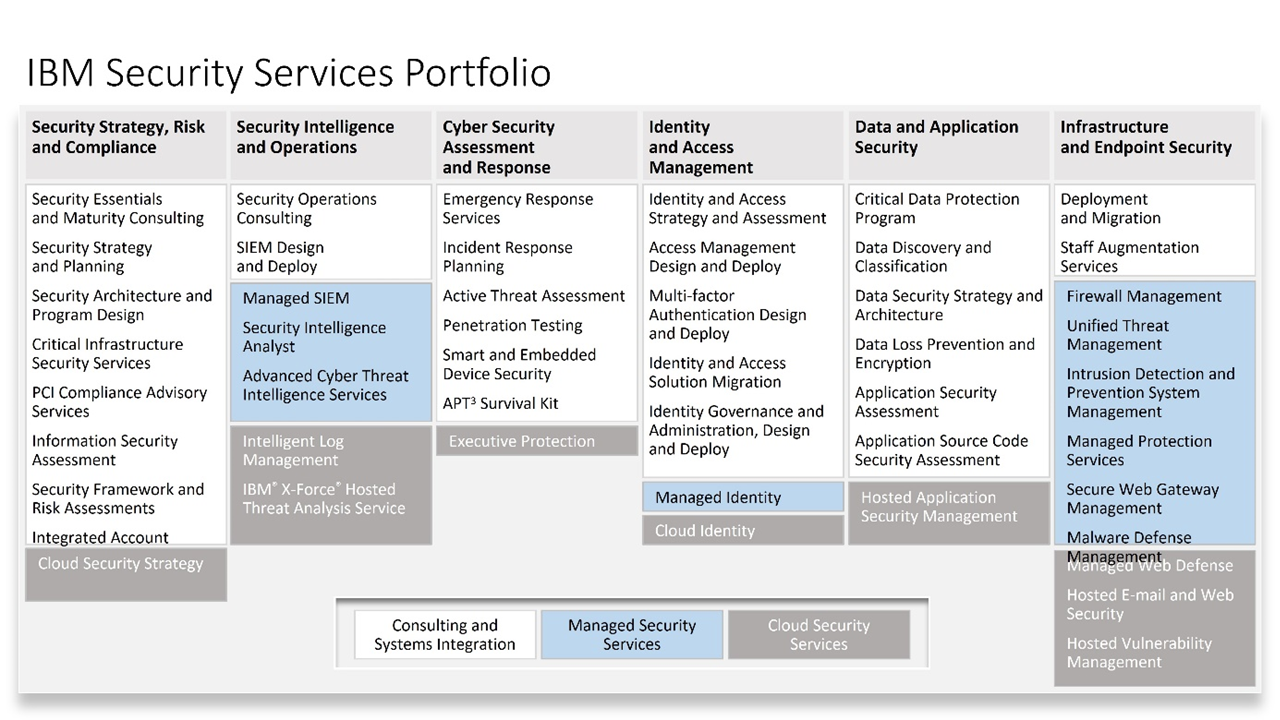
\includegraphics[width=\textwidth]{IBM-QRADAR}

\newpage
% \NUCwordcount{main}
\end{document}